\documentclass[10pt]{article}
\usepackage[a4paper,margin=1.4cm,top=1.2cm,bottom=1.2cm]{geometry}
\usepackage[table]{xcolor}
\usepackage{booktabs,graphicx,amsmath,enumitem,tabularx,array}
\usepackage[T1]{fontenc}
\usepackage{lmodern}
\setlength{\parindent}{0pt}\setlength{\parskip}{2.5pt}
\setlist{nosep,leftmargin=1.2em}
\pagestyle{empty}
\definecolor{acc}{RGB}{30,80,140}
\definecolor{boxbg}{RGB}{236,242,250}
\definecolor{warnbg}{RGB}{252,244,228}
\definecolor{good}{RGB}{190,232,190}\definecolor{fair}{RGB}{252,226,160}\definecolor{poor}{RGB}{244,182,176}
\newcommand{\head}[1]{\par\smallskip{\color{acc}\large\bfseries #1}\par\vspace{1pt}}
\newcommand{\key}[2][boxbg]{\par\colorbox{#1}{\parbox{\dimexpr\linewidth-2\fboxsep}{#2}}\par}
\newcommand{\rtHz}{$\sqrt{\text{Hz}}$}
\newcolumntype{L}[1]{>{\raggedright\arraybackslash}p{#1}}

\begin{document}
{\color{acc}\LARGE\bfseries Amplifier diagnostics from a single readout trace:}\\[1pt]
{\color{acc}\Large\bfseries what is new, and the physics it may reveal}\\[2pt]
{\small Skipper-CCD output amplifiers: PA03 (130\,K, boards 101/102) and LSM production modules DM07/09/10 (180\,K) \textperiodcentered{} 16 November 2026}

\key{\textbf{In short.} One raw trace of one channel (0.2\,s, no image, no charge) gives a setup-pickup number, the white
and 1/f noise of the output transistor, and timing flags, on one scale for every amplifier and test stand. A literature
check shows the individual techniques are established; what is new is the \emph{package} and its application across
test stands. Its scientific interest lies in a handful of \textbf{device-physics candidates} (gate-oxide traps,
single-trap telegraph noise, the buried-channel depth, amplifier light) that the same data expose. None is yet
confirmed; each needs one specific measurement, listed below.}

\head{1.\ The method, and where it stands in the literature}
\begin{itemize}
\item \textbf{Setup number:} the noise left after subtracting the repeating skip waveform, at 0.2--1\,kHz
  (\textmu V/\rtHz). Noise spectra are a standard diagnostic and pickup has been traced to grounding before [1]; we found
  no standard single number used to compare stands. \emph{New as a tool.}
\item \textbf{White vs 1/f from the CDS window:} fitting noise against window length through the exact CDS filter is the
  approach of Wüthrich et al.\ [1]; forming the windows in software from raw samples follows digital CDS and optimal
  filtering of skipper video [3,4]. \emph{Not new; a convenient single-trace implementation.}
\item \textbf{Flags:} telegraph noise from the kurtosis of the noise; an unsettled window from the in-window slope and the
  CDS offset. Simple, and we found no prior use of kurtosis for this. \emph{Minor.}
\item \textbf{Optimal window:} 5--8\,\textmu s at fixed readout time here; longer windows cost 9--32\,\%. This
  \emph{confirms} [1] ($\approx$9\,\textmu s; many short samples beat long windows); [2] found $\approx$20\,\textmu s on
  another device. \emph{Not new.}
\end{itemize}

\head{2.\ What the setup numbers show}
\begin{minipage}[t]{0.47\linewidth}\vspace{0pt}\footnotesize
\begin{tabularx}{\linewidth}{@{}Xr@{}}\toprule
setup number, 0.2--1\,kHz (\textmu V/\rtHz) & \\\midrule
PA03 board 101, October (0.2\,s traces) & \cellcolor{poor}48.8\\
PA03 board 101, Nov 10--12 (after cabling) & \cellcolor{poor}34.8\\
LSM ACM106 / ACM109, typical & \cellcolor{fair}5--15\\
LSM ACM110, quietest & \cellcolor{good}2.6--4.2\\
PA03 board 102, no charge & \cellcolor{good}1.5--1.6\\\bottomrule
\end{tabularx}
\end{minipage}\hfill
\begin{minipage}[t]{0.50\linewidth}\vspace{0pt}\small
\begin{itemize}
\item The cabling change cut board 101's pickup by 29\,\% (equal-length traces); images agree: shared noise 25\,\% $\to$
  5\,\%, ch0/ch1 read noise $-$30\,\%.
\item \textbf{The images no longer feel it:} board 101's 500-skip images (0.144--0.173\,e) sit at 0.84--0.89 of the
  white-averaging expectation. The CDS rejects most of this pickup; the per-skip noise sets the floor.
\end{itemize}
\end{minipage}

\head{3.\ Potential physics results}
{\footnotesize\renewcommand{\arraystretch}{1.15}
\begin{tabularx}{\linewidth}{@{}L{3.1cm}L{3.9cm}L{3.5cm}L{2.0cm}X@{}}\toprule
candidate & what we see & literature & status & what confirms it\\\midrule
\textbf{(a) Gate-oxide trap density of skipper output transistors} &
  $N_t\le1.1$--$2.4\times10^{16}$\,eV$^{-1}$cm$^{-3}$ on all 17 amplifiers, the same on PA03 (130\,K) and LSM (180\,K)
  (McWhorter model) &
  McWhorter model and CCD 1/f--trap links are classic [5]; we found \textbf{no trap density published for skipper
  amplifiers} & upper limit; method untested on an open input &
  window fit on an open input (expect no 1/f); the same module at two temperatures ($S_{1/f}\propto kT\,N_t$)\\
\textbf{(b) Single-trap telegraph noise} &
  ACM109 ch1: kurtosis 2.7, 1/f corner 334\,kHz; PA03 101 ch2: episodes in 1 of 127 traces &
  telegraph noise is well studied in small CMOS source followers; large CCD amplifiers are expected to be 1/f-limited &
  candidate (one LSM trace) &
  many traces; histogram of the two levels: step size and dwell times $\Rightarrow$ trap energy and depth vs temperature\\
\textbf{(c) Buried-channel depth from reset charge injection} &
  2.1--2.4\,fF/V, the same on all four PA03 CCDs $\Rightarrow$ depth $\approx$0.6\,\textmu m (0.3--0.9); process recipe
  predicts 0.5--0.7 &
  charge injection and reset feedthrough are well known; we found \textbf{no depth extracted this way} (usually C--V or
  SIMS) & model: assumes half the charge reaches the node &
  RG edge slowed by an RC (the split); clock-line capacitance at the connector (oxide vs depth)\\
\textbf{(d) Implant-dose difference between CCDs} &
  a 0.85\,V channel-potential shift on CCD\_B ($\approx$0.6\,\% dose), from output ``knees'' in voltage scans &
  knees in output vs bias are standard; dose inference not found & indicative (multi-rail scan) &
  single-rail scans, $\pm$0.05\,V\\
\textbf{(e) Sense-node capacitance} &
  84--95\,fF on all 17 amplifiers (follower gain 0.85 assumed); 60--80\,fF of it is wiring and diffusion &
  conversion gain and kTC methods are textbook & model; kTC cross-check being redone &
  DC level of the video line (sets the follower gain)\\
\textbf{(f) Amplifier light} &
  PA03 101 ch2: $\sim$22\,e$^-$/pixel peak at the amplifier end of its register, decaying over $\sim$1300 columns, absent
  in 1\,s exposures; 2.5$\times$ ch0's blank-image charge &
  a known source of single-electron events, characterised by SENSEI [6] & observed; cause inferred &
  amplifier off (or lower VDD) during exposure\\
\textbf{(g) Charge during skipping at 180\,K} &
  LSM images 1.2--2.0$\times$ their trace expectation, with $\sim$1\,e$^-$/pixel in blank images &
  dark current vs temperature is standard; the effect on skipper peak width is rarely quantified & inference &
  LSM images at 130\,K; noise vs skips at both temperatures\\\bottomrule
\end{tabularx}}

\par\smallskip
\begin{minipage}[t]{0.49\linewidth}\vspace{0pt}
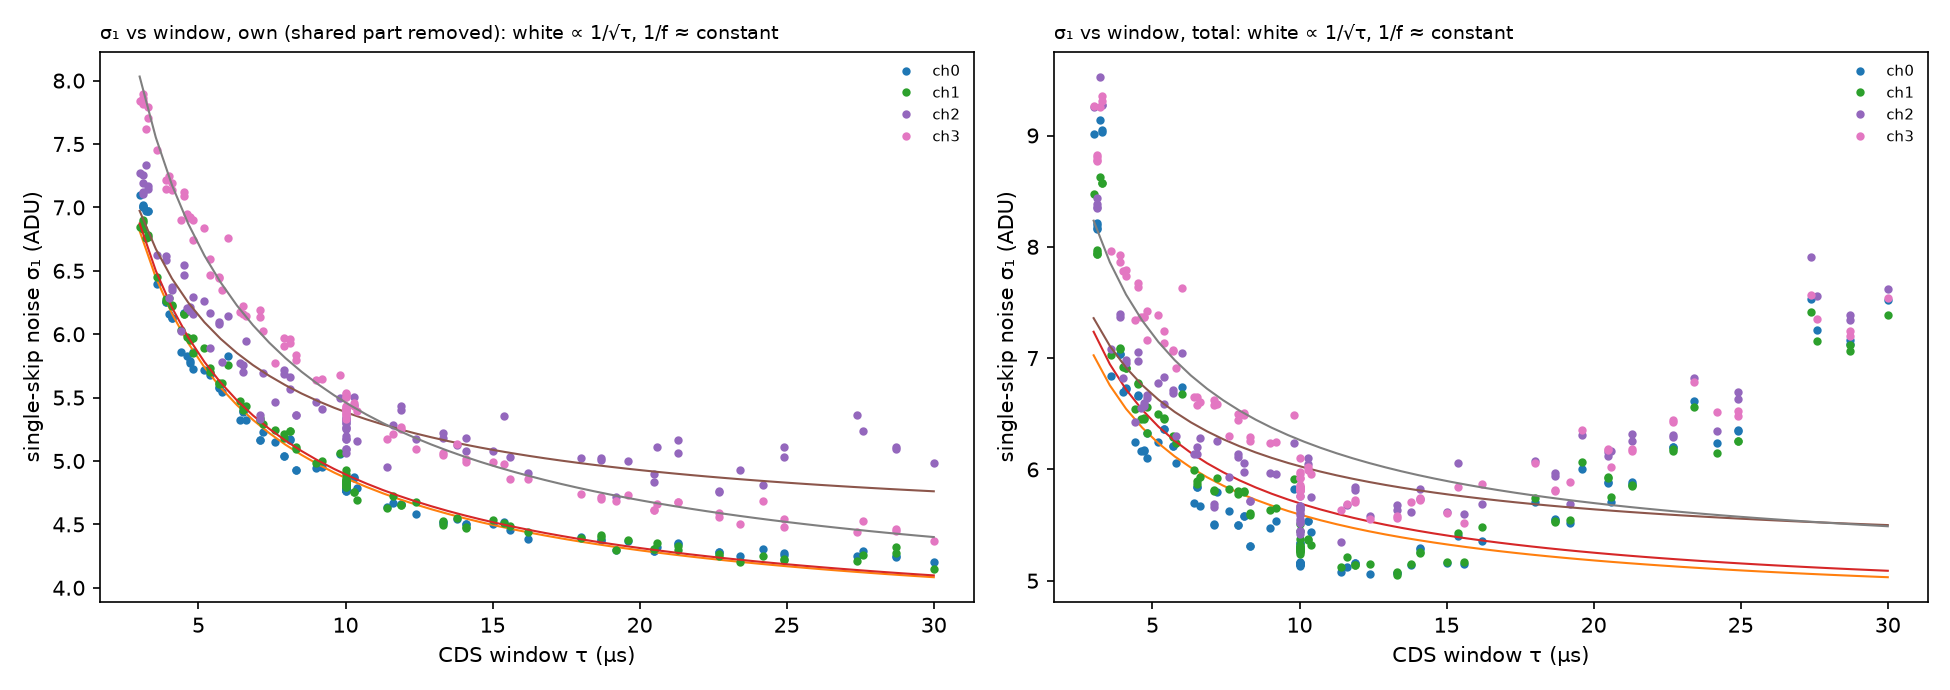
\includegraphics[width=\linewidth]{figures/oxide_traps_tau.png}\\[-2pt]
{\footnotesize (a) Single-skip noise against the CDS window (PA03, 100 strips) with white + 1/f fits. The part that does
not fall with the window is attributed to 1/f; the open-input control tests that attribution.}
\end{minipage}\hfill
\begin{minipage}[t]{0.49\linewidth}\vspace{0pt}
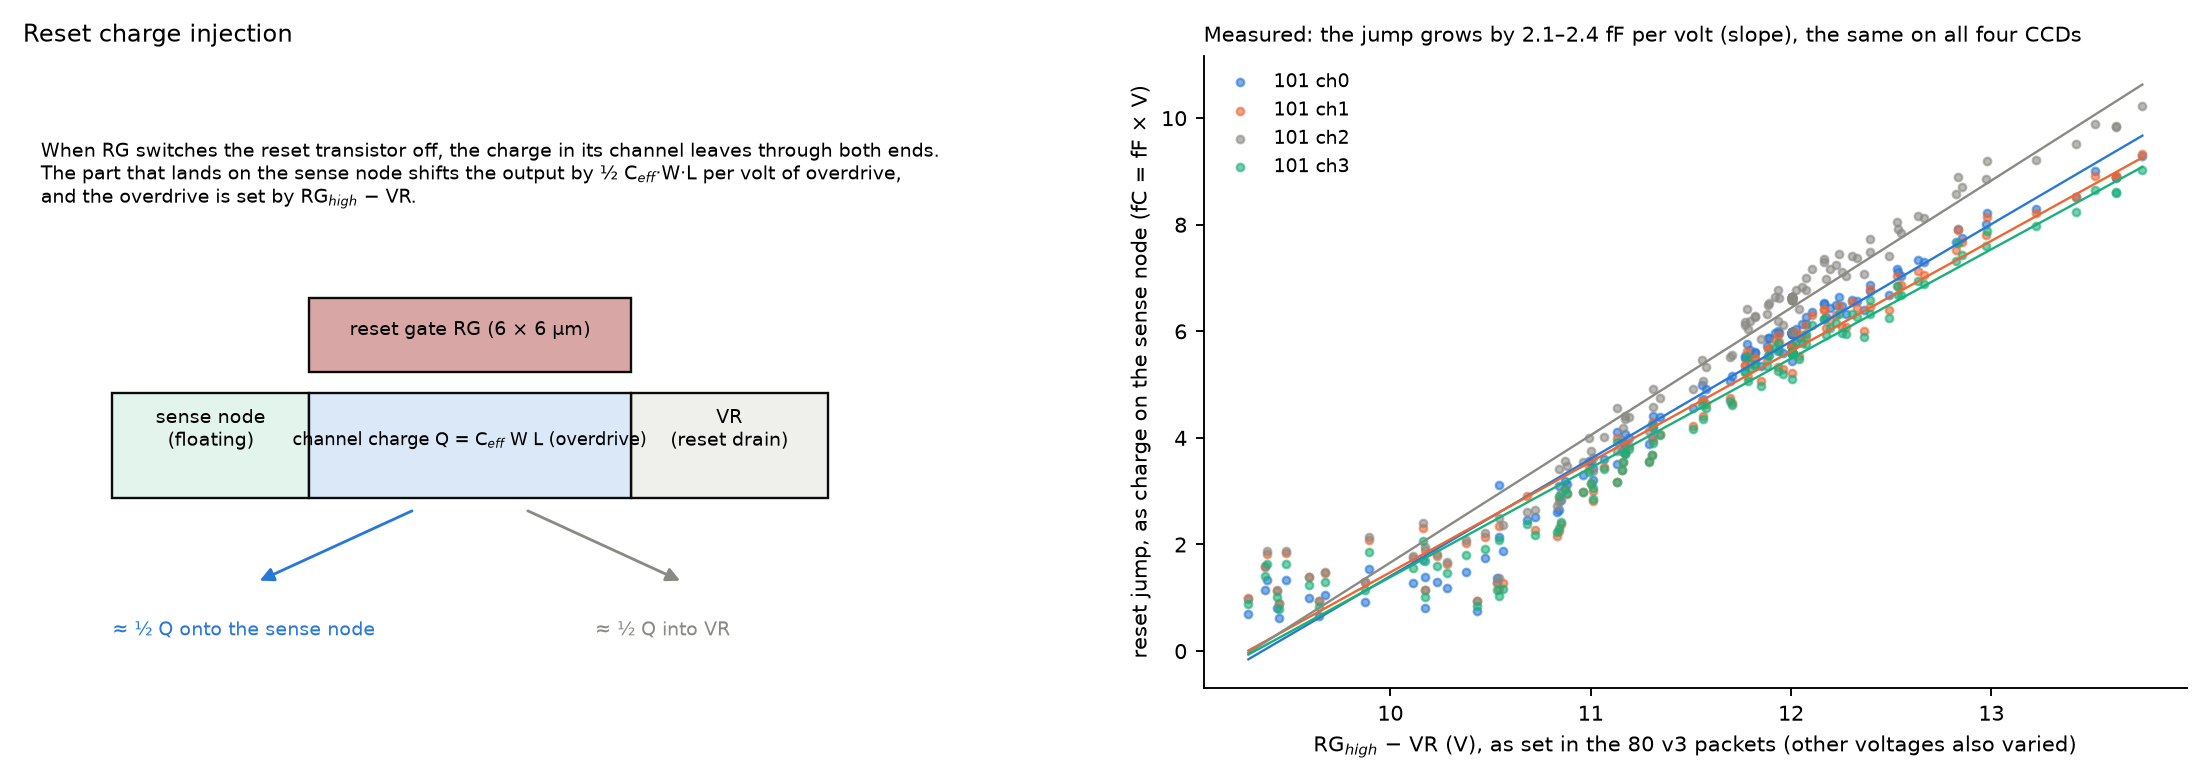
\includegraphics[width=\linewidth]{figures/charge_injection.png}\\[-2pt]
{\footnotesize (c) The charge injected at reset against RG$_\text{high}-$VR over 80 settings: the same slope on four
CCDs, which sets the depth of the buried channel through the oxide and silicon capacitances in series.}
\end{minipage}

\key{\textbf{The two most promising physics results, and why they would matter.}
\textbf{(a) Trap densities of skipper output transistors.} The 1/f noise of the output transistor is what limits a
single skip, and its gate-oxide trap density is the device parameter behind it. A per-amplifier number from routine
traces would let production modules be screened for oxide quality and compared across wafers and foundries, and would
make the 1/f floor predictable from a process parameter. We found no published value for skipper amplifiers.
\textbf{(c) A non-destructive buried-channel depth per CCD.} The depth sets the full-well, the transfer efficiency near
the surface and the coupling of every gate; it is normally known only from process simulation or a sectioned die. Here
it comes from operating data on every CCD, and the four PA03 CCDs agree with each other and with the recipe.
\textbf{Both hinge on one control each}: an open-input trace for (a), the reset charge split for (c).}

\head{4.\ Benefit, and the honest scope}
\begin{itemize}
\item \textbf{Practical value now:} setup debugging and run monitoring from one trace; screening production amplifiers
  (telegraph, timing: LSM board 109's windows are still settling, its CDS offsets reach $-1550$\,e); a common scale for
  comparing stands. DAMIC-M's underground characterisation of its 28 production modules [8] is a natural user.
\item \textbf{What is not new:} the window optimum and the white/1/f separation [1,2]; digital CDS [3,4]; kTC
  and conversion gain; correlated noise between modules and its software removal [7].
\item \textbf{Scope:} one PA03 module, one trace per LSM channel, two temperatures on different devices. Board 102's
  ch0--2 have transistors (no charge is sent to them), so results that treated them as bare electronics (the
  0.853\,ADU/\textmu V calibration, the pickup share of the reset feedthrough, the output-stage noise, the kTC estimate)
  are withdrawn or being redone. Absolute nV values use the design chain gain. The literature check covered abstracts
  and summaries, not full texts or collaboration notes.
\end{itemize}

\head{5.\ Next measurements, in order of physics payoff}
\textbf{(1)} trace with an open input (validates or kills (a)); \textbf{(2)} one module at two temperatures (trap scaling,
telegraph dwell times, (g)); \textbf{(3)} RC-slowed RG edge and one clock-line capacitance (firms up (c)); \textbf{(4)} DC
level of the video lines (e); \textbf{(5)} amplifier off during exposure (f); \textbf{(6)} more LSM traces per channel (b).

{\scriptsize\par\smallskip\textbf{References.}
[1] J.\ Wüthrich et al., Skipper CCD readout time optimization for astronomical applications, arXiv:2607.20126 (2026).
[2] Characterization and optimization of skipper CCDs for the SOAR Integral Field Spectrograph, PASP (2024), arXiv:2311.00813.
[3] A.\ Chierchie et al., Detailed modeling of the video signal and optimal readout of CCDs, Int.\ J.\ Circ.\ Theor.\ Appl.\ (2020), FERMILAB-PUB-20-319.
[4] Optimal CCD readout by digital correlated double sampling, arXiv:1510.09105.
[5] Characteristics of 1/f noise of the buried-channel CCD, Proc.\ SPIE 1071 (1989); McWhorter number-fluctuation model.
[6] SENSEI Collaboration, Characterization of single-electron events using a skipper-CCD, Phys.\ Rev.\ Applied 17, 014022 (2022), arXiv:2106.08347.
[7] DAMIC-M, The DAMIC-M Low Background Chamber, arXiv:2407.17872.
[8] DAMIC-M, First production of skipper-CCD modules for the DAMIC-M experiment, arXiv:2509.06943.}
\end{document}
